% Options for packages loaded elsewhere
\PassOptionsToPackage{unicode}{hyperref}
\PassOptionsToPackage{hyphens}{url}
%
\documentclass[
  12pt,
]{article}
\usepackage{amsmath,amssymb}
\usepackage{lmodern}
\usepackage{iftex}
\ifPDFTeX
  \usepackage[T1]{fontenc}
  \usepackage[utf8]{inputenc}
  \usepackage{textcomp} % provide euro and other symbols
\else % if luatex or xetex
  \usepackage{unicode-math}
  \defaultfontfeatures{Scale=MatchLowercase}
  \defaultfontfeatures[\rmfamily]{Ligatures=TeX,Scale=1}
\fi
% Use upquote if available, for straight quotes in verbatim environments
\IfFileExists{upquote.sty}{\usepackage{upquote}}{}
\IfFileExists{microtype.sty}{% use microtype if available
  \usepackage[]{microtype}
  \UseMicrotypeSet[protrusion]{basicmath} % disable protrusion for tt fonts
}{}
\makeatletter
\@ifundefined{KOMAClassName}{% if non-KOMA class
  \IfFileExists{parskip.sty}{%
    \usepackage{parskip}
  }{% else
    \setlength{\parindent}{0pt}
    \setlength{\parskip}{6pt plus 2pt minus 1pt}}
}{% if KOMA class
  \KOMAoptions{parskip=half}}
\makeatother
\usepackage{xcolor}
\usepackage[left=2cm,right=1.5cm,top=1cm,bottom=1.5cm]{geometry}
\usepackage{graphicx}
\makeatletter
\def\maxwidth{\ifdim\Gin@nat@width>\linewidth\linewidth\else\Gin@nat@width\fi}
\def\maxheight{\ifdim\Gin@nat@height>\textheight\textheight\else\Gin@nat@height\fi}
\makeatother
% Scale images if necessary, so that they will not overflow the page
% margins by default, and it is still possible to overwrite the defaults
% using explicit options in \includegraphics[width, height, ...]{}
\setkeys{Gin}{width=\maxwidth,height=\maxheight,keepaspectratio}
% Set default figure placement to htbp
\makeatletter
\def\fps@figure{htbp}
\makeatother
\setlength{\emergencystretch}{3em} % prevent overfull lines
\providecommand{\tightlist}{%
  \setlength{\itemsep}{0pt}\setlength{\parskip}{0pt}}
\setcounter{secnumdepth}{-\maxdimen} % remove section numbering
\usepackage{titling}
\pretitle{\begin{center} \includegraphics[width=6in,height=4in]{imagens//logoMD.jpg}\LARGE\\}
\posttitle{\end{center}}
\usepackage{colortbl}
\makeatletter
\setlength{\@fptop}{0pt}
\setlength{\@fpbot}{0pt plus 1fil}
\makeatother
\ifLuaTeX
  \usepackage{selnolig}  % disable illegal ligatures
\fi
\IfFileExists{bookmark.sty}{\usepackage{bookmark}}{\usepackage{hyperref}}
\IfFileExists{xurl.sty}{\usepackage{xurl}}{} % add URL line breaks if available
\urlstyle{same} % disable monospaced font for URLs
\hypersetup{
  hidelinks,
  pdfcreator={LaTeX via pandoc}}

\author{}
\date{\vspace{-2.5em}}

\begin{document}

\includegraphics[width=0.9\textwidth,height=\textheight]{imagens///logoMD.jpg}

\textbf{COMPONENTE CURRICULAR:} Física ~ ~ ~ \textbf{DATA}:
\_\_\_\_\_/\_\_\_\_/\_\_\_\_\_\_\\
\textbf{TURMA:} CICLO V ~ ~ ~ ~ ~ ~ ~ ~ ~ ~ ~ ~ \textbf{PROFESSOR:}
Jailson Duarte\\
\textbf{ALUNO(A):}
\_\_\_\_\_\_\_\_\_\_\_\_\_\_\_\_\_\_\_\_\_\_\_\_\_\_\_\_\_\_\_\_\_\_\_\_\_\_\_\_\_\_\_\_\_\_\_\_

\hypertarget{matemuxe1tica}{%
\section{\texorpdfstring{\centering MATEMÁTICA}{MATEMÁTICA}}\label{matemuxe1tica}}

\textbf{01.} A representação correta para o algarismo romano MMDCCCLXXVI
é:

A)27.456 ~ ~ B) 2.875 ~ ~ C) 12.445 ~ ~ D) 2.876 ~ ~ E) 28.513
\vspace{1cm}

\textbf{02.} Ao observarmos a bandeira do Brasil encontramos três formas
geométricas. São elas:

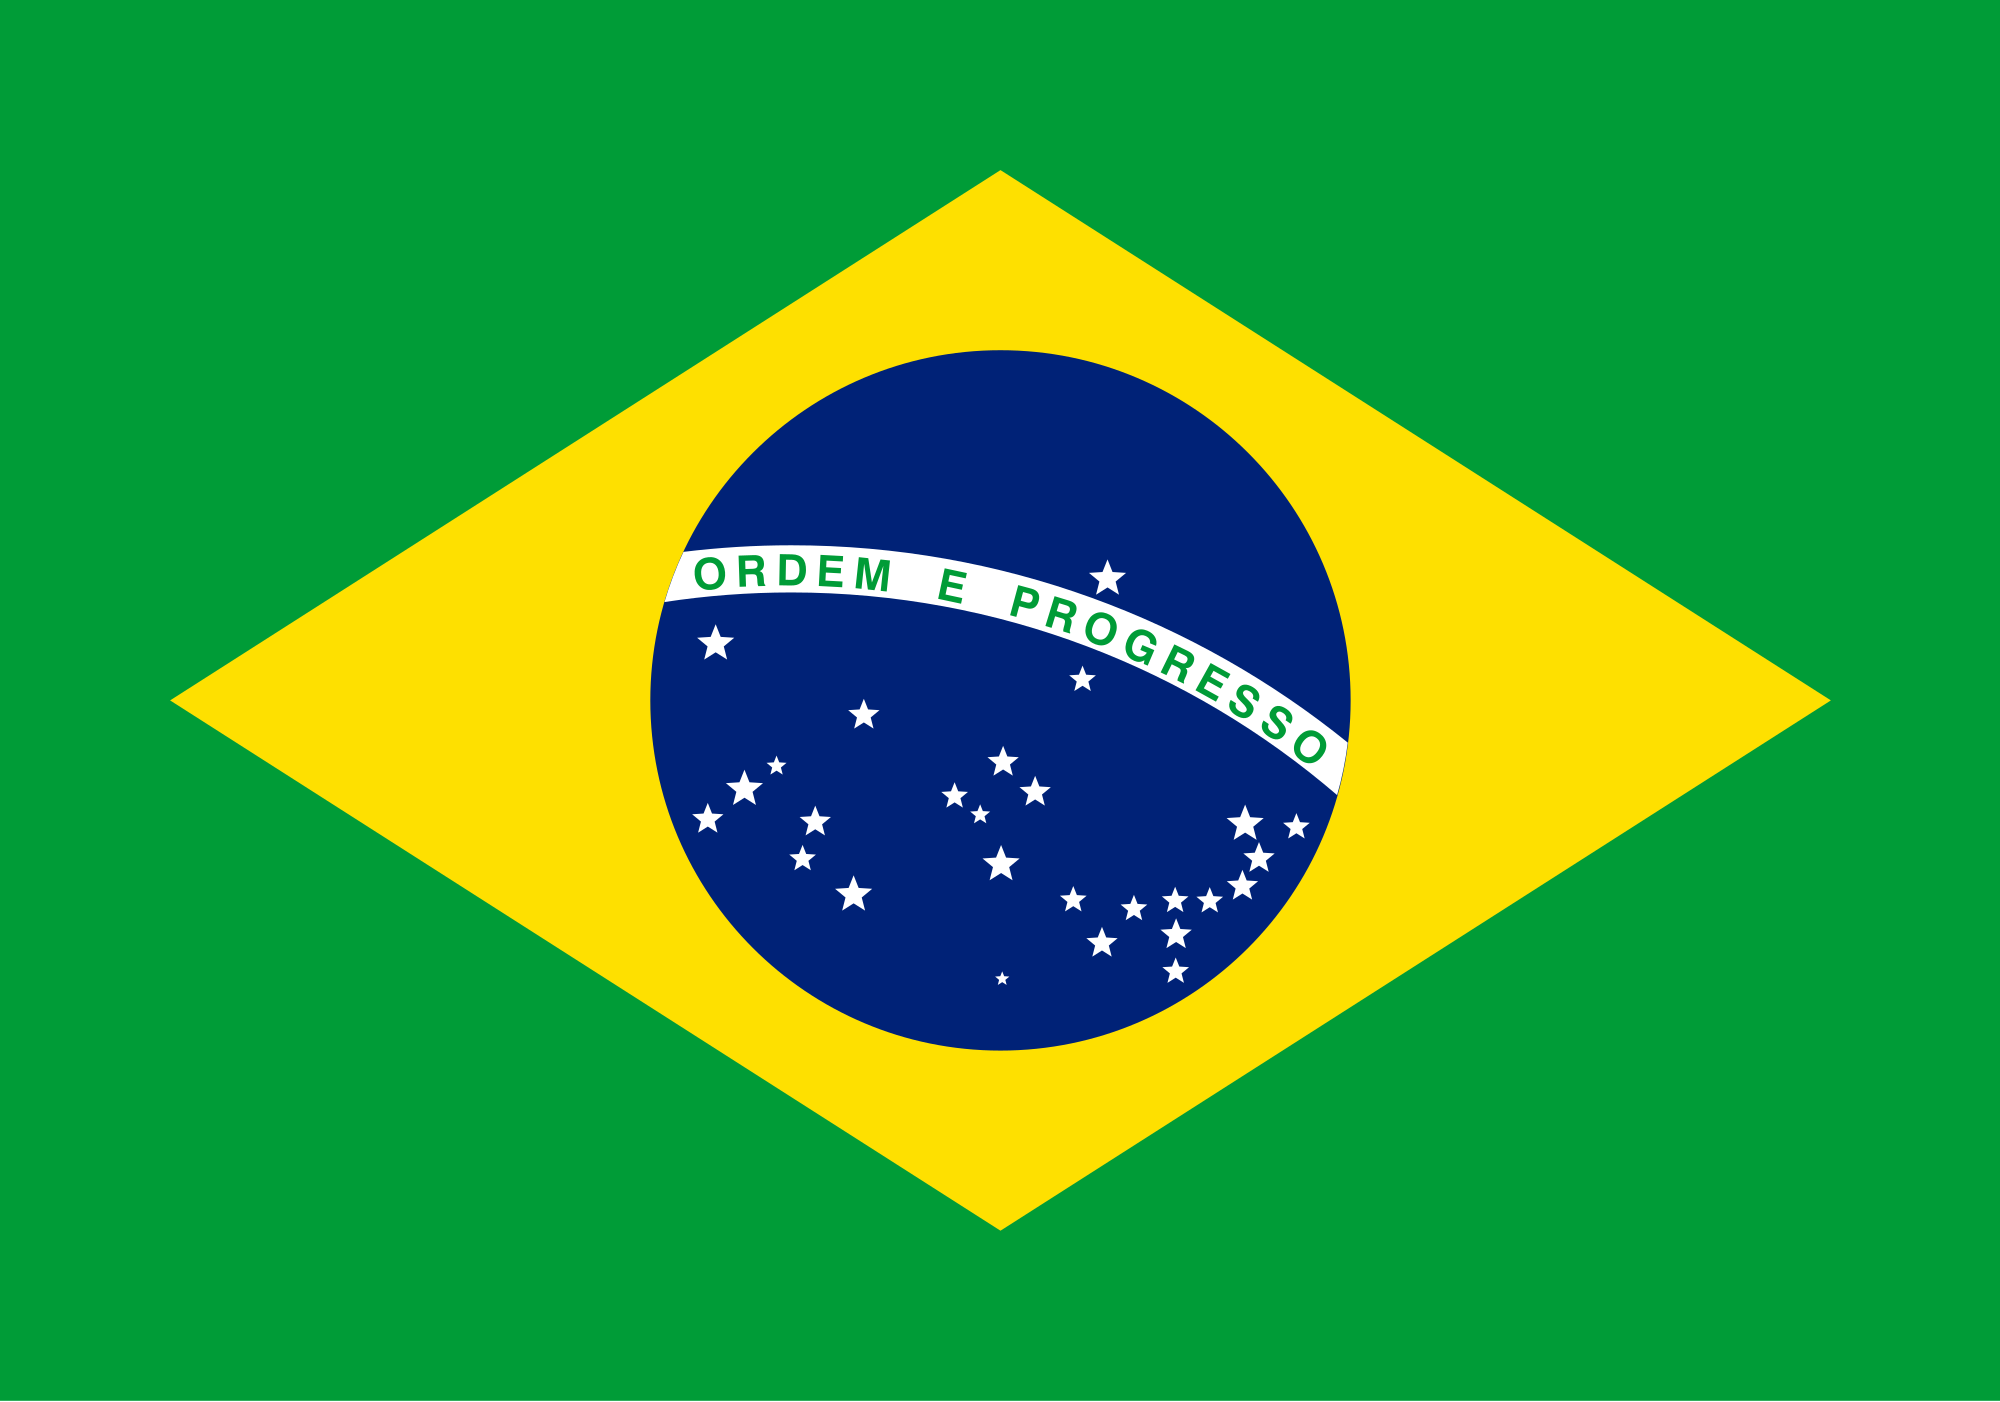
\includegraphics[width=0.4\textwidth,height=\textheight]{imagens///banderiraBrasil.jpg}

\begin{enumerate}
\def\labelenumi{\Alph{enumi})}
\item
  Quadrado, círculo e triângulo.
\item
  Reta, trapézio e triângulo.
\item
  Círculo, pentágono e losango.
\item
  Losango, círculo e retângulo.
\item
  Losango, quadrado e triângulo.
\end{enumerate}

\textbf{03.} Alberto sempre se atrasa nos encontros com sua namorada.
Numa semana em que eles combinaram de sair três vezes, sua namorada
registrou o tempo de atraso dele. No primeiro encontro ele se atrasou 22
minutos. No segundo, meia hora. Já no terceiro, ele se atrasou 44
minutos. Ao todo, o tempo de atraso de Alberto, nesses encontros, foi
de:

A)1 hora e meia ~ ~ B) 1 hora e 34 minutos C) 86 minutos

D)91 minutos ~ ~ E) 1 hora e 36 minuto

\vspace{1cm}

\textbf{04.} Agripino tinha um pacote com 50 chocolates. Distribuiu 3
para cada neto; além de dar um a sua esposa Clotilde. Sobraram 7
chocolates no final dessa distribuição. Logo, podemos concluir que
Agripino tem quantos netos?

\begin{enumerate}
\def\labelenumi{\Alph{enumi})}
\tightlist
\item
  3 ~ ~ B) 7 ~ ~ C) 14 ~ ~ D) 20 ~ ~ E) 5
\end{enumerate}

\vspace{0.8cm}

\textbf{05.} Um número, cujo antecessor é 234, é multiplicado por 3 e
somado ao sucessor de 132. Após a realização desses cálculos, conclui-se
que o resultado final se encontra na alternati va:

\begin{enumerate}
\def\labelenumi{\Alph{enumi})}
\tightlist
\item
  832 ~ ~ B) 833 ~ ~ C) 835 ~ ~ D) 837 ~ ~ E) 838
\end{enumerate}

\textbf{06.} Em uma hora, uma tartaruga percorreu 1.874 milímetros, e
manteve a constância na sua caminhada. Podemos concluir que em duas
horas ela percorre, em metros, o igual a:

\begin{enumerate}
\def\labelenumi{\Alph{enumi})}
\tightlist
\item
  1,874 ~ ~ B) 3,748 ~ ~ C) 18,74 ~ ~ D) 37,48 ~ ~ E) 187,4
\end{enumerate}

\textbf{07} Marcelo trabalha 22 dias por mês, como garçom. Como é um
restaurante frequentado por pessoas muito ricas, ele recebe uma boa
quantia em gorjetas. Em um determinado mês ele calculou que recebeu R\$
22,70 por dia de trabalho, somente em gorjetas. Sabendo que ele recebeu,
além das gorjetas, o seu salário fixo, de R\$ 705,60 e uma gratificação
(por bom trabalho) de R\$ 230,00, calculamos que ao final recebeu um
valor total de:

A)R\$ 1434,00 ~ ~ B) R\$ 1434,10 ~ ~ C) R\$ 1434,30

D)R\$ 1434,50 ~ ~ E) R\$ 1435,00

\vspace{0.8cm}

\textbf{08} O resultado da expressão numérica
\(725 \div 5 + 22 + 15 \times 12 + 16=\), é:

\begin{enumerate}
\def\labelenumi{\Alph{enumi})}
\tightlist
\item
  234 ~ ~ B) 143 ~ ~ ~ ~ C) 363 ~ ~ D) 608 ~ ~ E) 567
\end{enumerate}

\textbf{09} Um halterofilista faz diversos exercícios durante o dia. Ele
faz 6 séries de 50 repetições (6 x 50) de exercícios abdominais. Já o
resto dos exercícios (que totalizam 9), ele faz em 4 séries de 8
repetições (4 x 8) cada uma. Ao todo, quantas repetições ele faz em um
dia?

\begin{enumerate}
\def\labelenumi{\Alph{enumi})}
\tightlist
\item
  588 ~ ~ B) 589 ~ ~ C) 590 ~ ~ D) 591 ~ ~ E) 592
\end{enumerate}

\textbf{10} A escola Menino Jesus decidiu fazer um passeio com seus
alunos para um museu. Precisou alugar três ônibus para acomodá-los
confortavelmente. A escola levou 135 alunos e três professores, quantos
foram em cada ônibus, se foi dividido igualmente?

\begin{enumerate}
\def\labelenumi{\Alph{enumi})}
\tightlist
\item
  35 ~ ~ B) 46 ~ ~ C) 45 ~ ~ D) 50 ~ ~ E) 28
\end{enumerate}

\end{document}
